\subsection{Multi-source Even Data Fraction}
We extend the single source assignment to multi-source assignment problem\cite{jia2010scheduling}.  According to each processor, we concentrate on the processors' geographical location $P_{i}$, data fraction assigned $\alpha_{i}$.
\\
Assuming the data fraction is even.  For example, the workload is unit $1$ and there are $k$ different data injection options.  So each data injection is assigned $\frac{1}{k}$ workload.
From the data injection position relationship we consider three different situations :
\begin{itemize}
\item $G_{L}$ : Data injection positions consist of a subgraph of $G$.
\item Data injection processor doesn't connect with each other.
\item Data injection positions are mix of $1$ and $2$.
\end{itemize}

\subsubsection{Situation \uppercase\expandafter{\romannumeral1}}
If the data injection positions consist of a subgraph of $G$, we use $G_{L}$ to present it.
\begin{figure}[!ht]
\centering
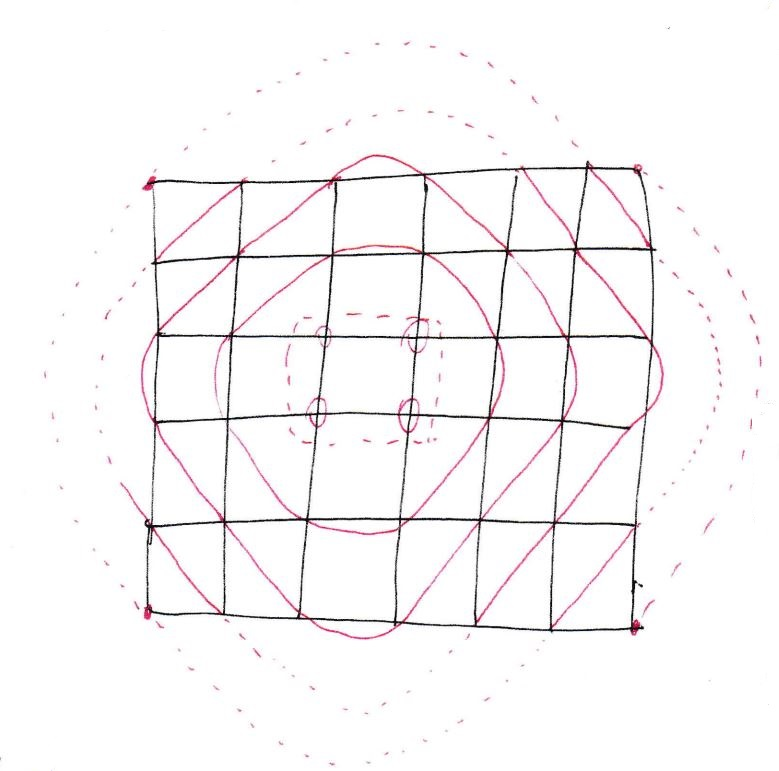
\includegraphics[width=0.5\columnwidth]{figure/subgraph1.jpg}
\caption{Data injection consists of a subgraph of $G$}
\label{fig:subgraph1}
\end{figure}

\begin{figure}[!ht]
\centering
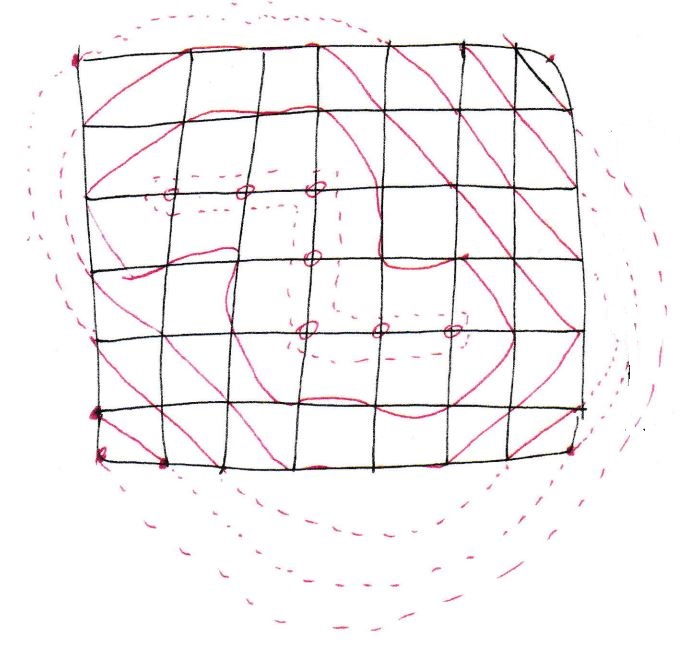
\includegraphics[width=0.5\columnwidth]{figure/subgraph2.jpg}
\caption{Data injection consists of a subgraph of $G$}
\label{fig:subgraph2}
\end{figure}
\newpage

\Fig{subgraph1} and \Fig{subgraph2} illustrate two situations that the data injections consist of subgraph $G_{data}$ of the whole graph $G$. 

The heuristic algorithm tackling this scenario is divided into two stages, $global_{s}$ and $local_{s}$ stages.

\begin{itemize}
\item $global_{s}$ : We collapse the data injection processors into one ``big" equivalent processor $P_{eq}$ \cite{robertazzi1993processor}.
\item $local_{s}$ : Re-distributing workload between the data injection processors.
\end{itemize}

For example, \Fig{subgraph1}'s \textbf{\textit{flow matrix}} is :

\begin{equation}
{
\left[ \begin{array}{cccccc}
4 & 8 & 12 & 10 & 6 & 2\\
1 & -1 & 0 & 0 & 0 & 0\\
0 & \sigma-1 & 1 & 0 & 0 & 0\\
0 & \sigma-1 & \sigma & 1 & 0 & 0\\
0 & \sigma-1 & \sigma & \sigma & 1 & 0\\
0 & \sigma-1 & \sigma & \sigma & \sigma & 1\\
\end{array} 
\right ]} \times \left[ \begin{array}{c}
\alpha_{0} \\
\alpha_{1} \\
\alpha_{2} \\
\alpha_{3} \\
\alpha_{4} \\
\alpha_{5}
\end{array} 
\right ] = \left[ \begin{array}{c}
1 \\
0 \\
0 \\
0 \\
0 \\
0
\end{array} 
\right ]
\end{equation}
The simulation result illustrates as follows:

\begin{figure}[!ht]
\centering
\includegraphics[width=1\columnwidth]{figure/vo_sub1.eps}
\caption{Speedup vs $\sigma$}
\label{fig:vo_sub1}
\end{figure}

This simulation says the best performance happens on value $\sigma \leq 0.05$, which hits about $40$ times speedup.  If $\sigma \approx 1$, the network achieves almost $12$ times performance. 

\newpage
\subsubsection{Situation \uppercase\expandafter{\romannumeral2}}
The data injections don't consist of a subgraph of $G$.  
Jia \cite{fortune1995voronoi} propose an algorithm to utilize the nearest data injection principle to tackle this scenario.  In the dividable load intricate applications, for example, big file transmission, GPU scientific computation \cite{krevat2002job} or Hadoop job, the total job finish time depends on the last piece, that is, which spends the longest sub-job finish time.  \\
Our objective function is to utilize less processors to achieve the same finish time.  \\
\Fig{voronoi_even_cells} shows $10$ voronoi cells division and \Fig{voronoi_even_speedup} figures out the speedup of each cells.\\
\begin{figure}[!ht]
\centering
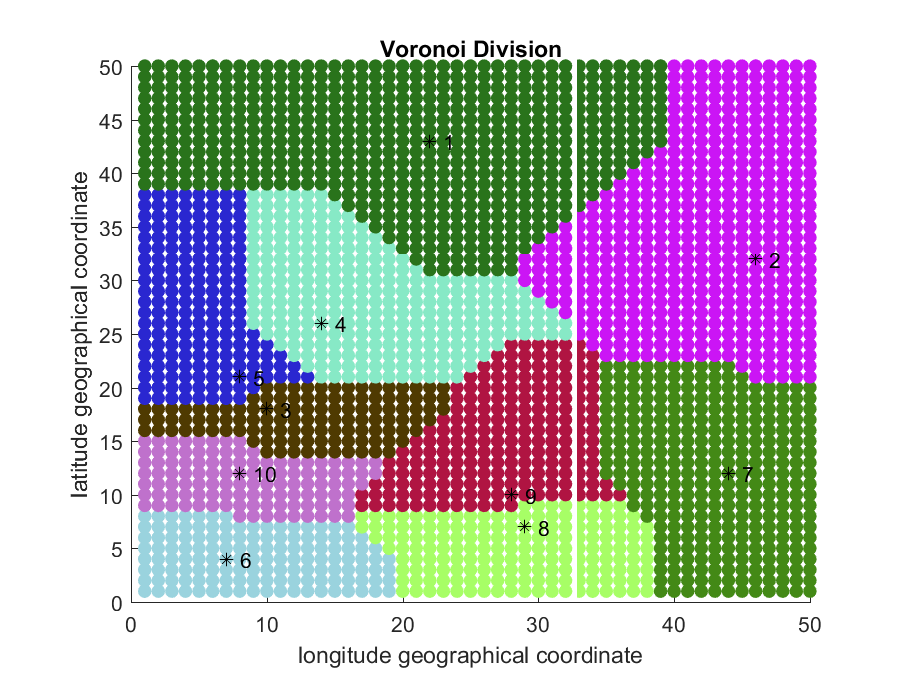
\includegraphics[width=1\columnwidth]{figure/voronoi_even_cells.eps}
\caption{$10$ Voronoi Cells}
\label{fig:voronoi_even_cells}
\end{figure}

\begin{figure}[!ht]
\centering
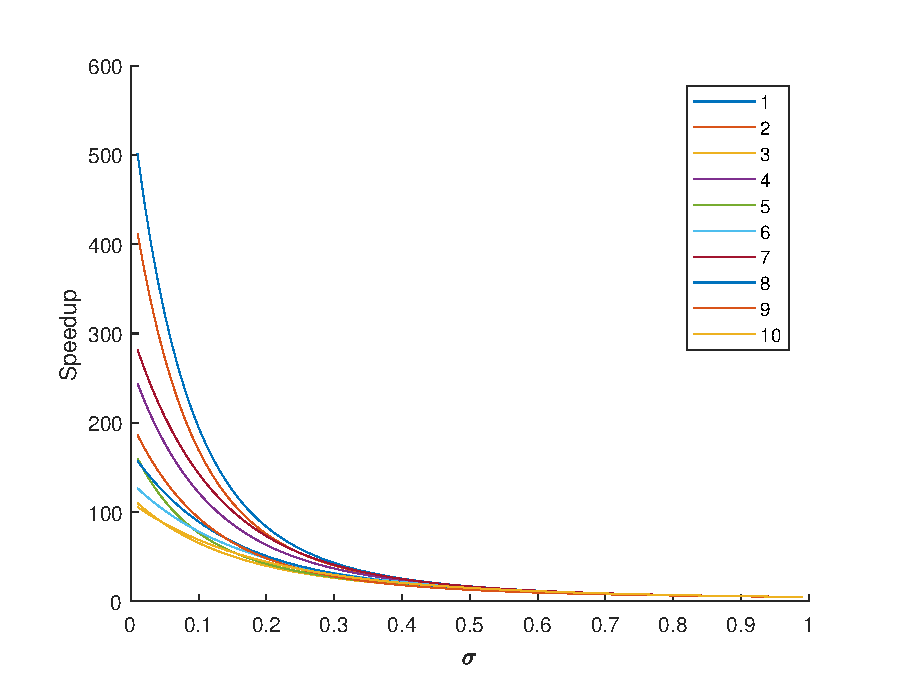
\includegraphics[width=1\columnwidth]{figure/voronoi_even_speedup.eps}
\caption{$10$ Voronoi Cells's speedup curves}
\label{fig:voronoi_even_speedup}
\end{figure}
\newpage 

The heuristic algorithm is named as \textbf{\textit{Reduced Voronoi Division Algorithm}}:

\begin{algorithm}
\caption{Reduced Voronoi Diagram Algorithm(RVDA)}
\begin{algorithmic} 

\floatname{algorithm}{Procedure}
\renewcommand{\algorithmicrequire}{\textbf{Input: $n$ data injection position}}
\renewcommand{\algorithmicensure}{\textbf{Output: $n$ reduced Voronoi division}}

\STATE Calculate $n$ Voronoi cells with Manhattan distance.
\STATE Calculate $n$ radius $R_{i}$ of $n$ Voronoi cells.
\STATE Set $R_{min} = \min {R_{i}}$
\WHILE{$1 \leq i \leq n$}
\STATE Calculate the Reduced Voronoi cells by setting the $R_{i} = R_{min}$ in each cell.
\STATE Calculate Voronoi cell's flow matrix $A_{i}$.
\STATE $ i = i + 1$
\ENDWHILE
\STATE Display each reduced Voronoi cells
\STATE Illustrate each reduced Voronoi cells' speedup curves
\end{algorithmic}
\end{algorithm}
\newpage

\Fig{voronoi_even_cells_save} and \Fig{voronoi_even_speedup_save} show the algorithm's result and speedup curves.  The algorithm keeps the same running time yet save about $30 \%$ processors.

\begin{figure}[!ht]
\centering
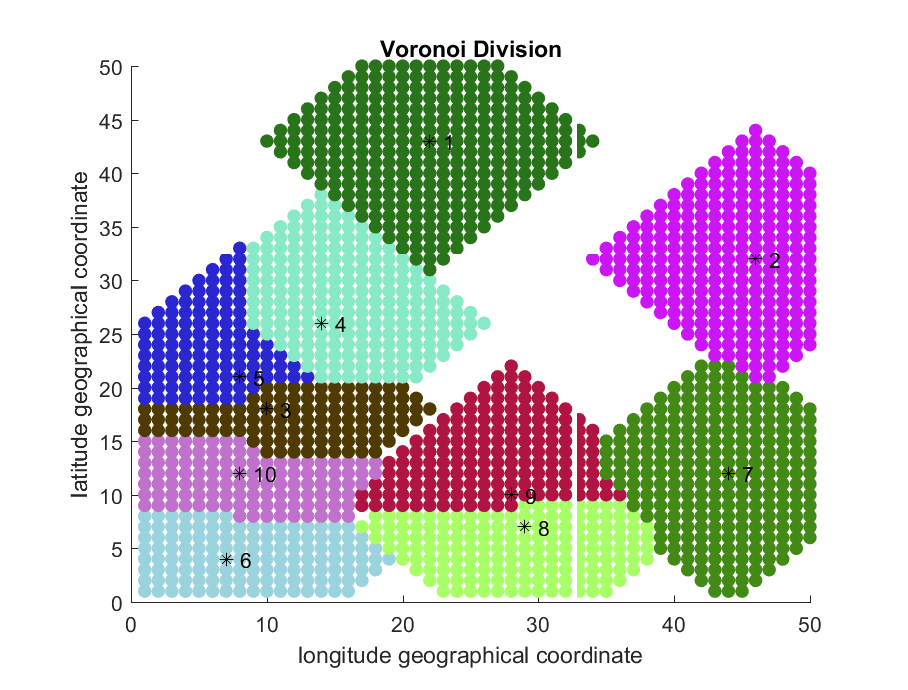
\includegraphics[width=1\columnwidth]{figure/voronoi_even_cells_save.eps}
\caption{$10$ Voronoi Cells}
\label{fig:voronoi_even_cells_save}
\end{figure}

\begin{figure}[!ht]
\centering
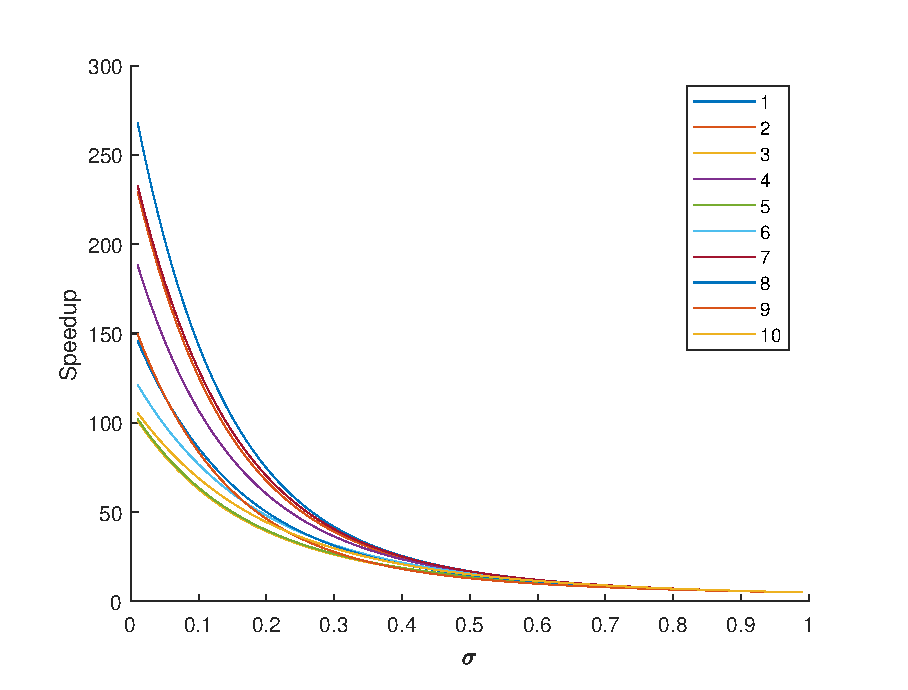
\includegraphics[width=1\columnwidth]{figure/voronoi_even_speedup_save.eps}
\caption{$10$ Voronoi Cells's speedup curves}
\label{fig:voronoi_even_speedup_save}
\end{figure}

\Fig{voronoi_even_speedup} shows $\sigma < 0.2$, the ratio $\frac{max speedup}{min speedup} = \frac{500}{100} = 5$ and \Fig{voronoi_even_speedup_save} shows the ratio is $\frac{max speedup}{min speedup} = \frac{270}{100} = 2.7$.  \\
It displays that $10$ pieces of processor cluster's equal computation is more balanced than initiation setting, and the whole cluster finishes tasks with the same time by less processors.

\newpage
After $1000$ round random sampling data injection position, we obtain the average saved processors result in \Fig{voronoi_save}.

\begin{figure}[!ht]
\centering
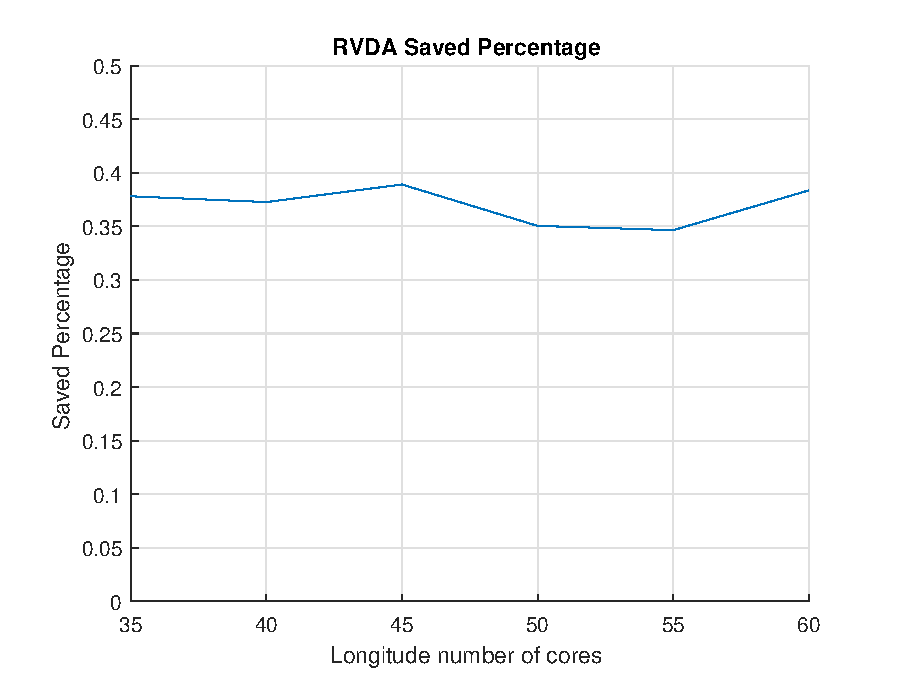
\includegraphics[width=1\columnwidth]{figure/voronoi_save.eps}
\caption{Reduced Voronoi Division Algorithm average processors' percentage}
\label{fig:voronoi_save}
\end{figure}

From \Fig{voronoi_save}, it shows the average percentage of saved processor is about $35 \%$.
\newpage

\newpage
\subsubsection{Situation \uppercase\expandafter{\romannumeral3}}
